\documentclass[10pt]{article}
\usepackage[preprint]{rlj}
\usepackage{graphicx,booktabs}
\title{Exploration, memory and action reachability in student-scale ARC-AGI-3 agents}
\setrunningtitle{WitsC: DQN and PPO for ARC-AGI-3}
\author{Nathan Le Roux, Tafara Chibanda, Samuel Snyman, Joshua Snyman}
\emails{\{2717495,2683459,2677730,2677722\}@students.wits.ac.za}
\affiliations{University of the Witwatersrand --- COMS4061A/COMS7071A}
\begin{document}
% No makeCover: the course explicitly disables the RLC cover page.
\maketitle
\begin{abstract}
We investigate convolutional DQN and PPO agents for interactive ARC-AGI-3 puzzles under a limited training budget. A shared interface represents four visual frames and a discrete click lattice. We evaluate episodic novelty and action-history interventions independently for both algorithms. On one development game, sampled PPO with novelty completes a level in 28/60 evaluation episodes compared with 5/60 for its baseline. DQN with 30\% evaluation exploration completes a level in 42/60 baseline episodes; its trained novelty and no-change-memory variants regress to 13/60 and 25/60. Neither algorithm solves a full game in the audited development evaluations. Visual replay identifies an action representation that cannot reach any second-level tile; a finer grid repairs reachability but does not improve first-level completion under the same budget. These results distinguish policy activity, exploration and representational feasibility from reliable reasoning. We provide self-contained competition notebooks, original evaluation evidence and explicit limitations. Code: \url{https://github.com/TafaraC/RL_Project}.
\end{abstract}

\section{Problem and research questions}
ARC-AGI-3 requires an agent to infer unfamiliar controls and goals through sequential interaction with visual games. The agent receives public observations and legal actions, but no explicit rules or complete latent state. We ask whether modest reinforcement-learning agents can discover useful behaviour, whether novelty and short memory improve it, and whether the action representation itself prevents progress. This is an empirical student project, not a claim of a new RL algorithm or general puzzle solver.

We use DQN as the course-based value-learning algorithm and PPO as the second, policy-gradient algorithm. The shared scaffold and libraries reduce implementation duplication; the novelty, reset, rollout-memory and submission logic were adapted and tested for this project. Related methods are DQN's replay and target-network approach \citep{mnih2015}, PPO's clipped objective \citep{schulman2017}, and generalized advantage estimation \citep{schulman2016}. Our exact-frame counter is a simple exploration heuristic, not a learned density model.

\section{Environment formulation and interface}
The underlying game is partially observable: the four-frame history is an approximate state representation, not a proven Markov state. Each 64-by-64 frame has 16 colour indices, represented as 16 one-hot planes. Four post-action frames produce 64 input channels; missing history is zero-padded. Only the newest frame in each public response is appended. We do not use engine internals as policy features.

Seven simple actions (RESET, ACTION1--5 and ACTION7) and an $8\times8$ lattice of click centres give 71 actions. ACTION6 carries click coordinates; its legality activates all lattice cells. The finer $16\times16$ representation has 263 actions. Available-action masks come from the public interface. This discretisation is computationally convenient but can remove necessary actions.

The Gymnasium adapter returns the latest frame, action mask and progress information. WIN terminates; 1,000 consumed actions truncate. GAME\_OVER triggers a reset inside the same budgeted episode, clearing visual/action history while retaining the agent's parameters. The initial reset is excluded from this budget, but internal resets count. A selected RESET also clears history. The official framework counts the initial reset, so our notebook permits 1,001 total calls to reproduce this convention. Training decisions and consumed actions are consequently distinct.

Training reward is $+1$ per completed level, $+5$ on WIN, $-0.05$ on death and $-0.002$ per action. These rewards support learning only. They are not official relative human action efficiency scores. All reported development success rates use observed level completion, include unsuccessful episodes and are explicitly local. No official Kaggle score was available when preparing this report.

\section{Learning algorithms}
\subsection{DQN}
DQN learns an action-value function $Q_\theta(h,a)$ from replayed transitions. Its masked Bellman target is $y=r+\gamma(1-d)\max_{a'\in\mathcal A(h')}Q_{\bar\theta}(h',a')$, with a separate target network and Huber loss. True terminals suppress bootstrapping; action-budget truncation retains a bootstrap. Epsilon-greedy behaviour explores legal actions during training. Network parameters persist across episodes; replay is a training resource and is absent from inference. The target is copied periodically to stabilise learning.

The CNN uses three convolutional layers with 32, 64 and 64 channels, kernels 5, 3 and 3, stride 2, followed by a 512-unit fully connected layer and action outputs. Adam learning rate is $2.5\times10^{-4}$, discount 0.99, batch size 64, learning starts after 1,000 transitions, updates occur every four decisions and target copies every 1,000 gradient updates. Epsilon decays from 1 to 0.05 over 50,000 decisions. The implementation packs binary observations to limit replay storage. Historical baseline configurations and later improvement configurations are preserved with the evidence; hardware differs from PPO.

\subsection{PPO and its update loop}
PPO learns a categorical policy and scalar value on the same CNN, with one additional value output. During training it samples a legal action and retains the observation, mask, old log probability, reward and value. After 128 transitions, generalized advantage estimation computes
\begin{equation}
\delta_t=r_t+\gamma V(h_{t+1})-V(h_t),\qquad
\hat A_t=\delta_t+\gamma\lambda\hat A_{t+1},
\end{equation}
with terminal/bootstrap and reset-boundary masks applied separately. True terminals use zero next value; truncations bootstrap but stop advantage recursion across episode resets. Advantages are normalised over the rollout.

With $\rho_t=\pi_\theta(a_t|h_t)/\pi_{\mathrm{old}}(a_t|h_t)$, PPO minimises the negative mean of $\min(\rho_t\hat A_t,\mathrm{clip}(\rho_t,0.8,1.2)\hat A_t)$, plus $0.5$ times value mean-squared error, minus $0.01$ times policy entropy. Four epochs use minibatches of 32. Adam learning rate is $3\times10^{-4}$, $\gamma=0.99$, $\lambda=0.95$ and gradient norm is capped at 0.5. Old masks and probabilities stay fixed during each update. Packed rollouts store the exact augmented observations, so a history intervention cannot silently change the likelihood-ratio inputs. The partial final rollout is updated before saving.

Evaluation freezes all weights. PPO samples from its categorical policy; greedy evaluation is a secondary diagnostic. DQN's principal historical stochastic diagnostic uses epsilon 0.3, which was selected after inspecting development behaviour. This makes exploration part of the evaluated policy and introduces selection bias. We do not compare greedy DQN against sampled PPO as if they used identical decision rules.

\section{Experimental protocol}
The pre-recorded shuffle (seed 2026) selects development games dc22, ft09, g50t and m0r0 from 25 public games; cd82, tr87 and vc33 are reserved for final transfer. Each development game is trained separately with independent training seeds 0, 1 and 2 and a requested 50,000 decisions. The runner finishes its last episode, yielding approximately 50,600--51,000 actual decisions per run. Each sampled development checkpoint has 20 evaluation rollouts, with sampling seeds 100--119 and 1,000 actions. The wrapper seeds action selection, not game layout generation.

The principal comparison comprises three DQN stages and five PPO conditions. Each seed is an independently trained model; the 60 pooled rollouts per condition do not constitute 60 independent models. Individual seed results are shown rather than unsupported significance claims. Frozen-policy evaluations reuse trained development games and cannot establish generalisation. The random reference in Nathan's recovered archive has three seeds, 20 episodes each, on ft09. Earlier report-only results for other random games are not promoted to verified measurements.

PPO training used Windows/Python 3.14.3, PyTorch 2.14.1+cu130 and an RTX 3050 Laptop GPU. DQN improvement runtime records specify Python 3.12.10 and CPU execution, despite a CUDA-capable PyTorch build. Both use arcengine 0.9.3 and arc-agi 0.9.9. GPU neural inference/training does not move the Python game engine to the GPU. Unequal hardware prevents interpreting elapsed time as a clean algorithmic efficiency comparison.

\section{Iterative improvements and development evidence}
\subsection{DQN: exploration and no-change memory}
The baseline's greedy behaviour repeatedly selects a small set of actions. Training completion therefore need not indicate a capable greedy policy: exploration noise may perform the useful actions. First, a training-only first-visit screen bonus of 0.01, capped at 0.5 per episode, encourages visual exploration. Second, a per-screen memory records actions whose latest frame did not change and masks them on returning to that screen. If all legal actions would be excluded, the legal mask is restored. This intervention uses public screen history, persists within an episode and changes action selection without adding a learned recurrent model.

The memory-trained DQN condition disables novelty, so it is a separate intervention, not a demonstrated cumulative novelty-plus-memory improvement. The archive also contains combined novelty-plus-memory training on ft09, but no corresponding complete evaluation; it is excluded from performance claims. Applying memory at evaluation to baseline DQN yields 47/60 ft09 completions versus 42/60 without it, while the separately memory-trained condition gives 25/60. Thus the small post-hoc gain does not establish that memory training improves DQN. Novelty training gives 13/60, also below baseline. Historical evaluation folders lack saved evaluation configurations; epsilon/memory settings are inferred from their names and associated scripts, a reproducibility limitation.

\subsection{PPO: novelty, then explicit action history}
Baseline sampled PPO rarely completes the first ft09 level. We add a diminishing bonus $0.01/\sqrt{N(s)}$ for the exact newest visible screen, capped at 0.5 per episode. Counts persist across internal death resets but reset at the next outer episode. Unlike DQN's first-visit bonus, repeated screens retain decreasing reward. The intervention increases pooled ft09 level completion from 5/60 to 28/60, but the result is dominated by seed 2, which completes 20/20 compared with 4/20 for each other seed.

Visual diagnosis motivates a second intervention: explicit previous-action, repeated-action and unchanged-screen history. Sixteen binary planes encode the previous simple action (seven planes), the prior click cell (one), and two four-step saturated thermometer counters (eight). These are prepended to the four visual frames, yielding 80 channels. Memory clears on resets and continues across level transitions. The reward and PPO objective are unchanged. A finer-grid novelty-only control isolates the memory contribution; a memory-only condition removes novelty. Memory plus novelty reaches only 3/60 compared with the matched control's 10/60; memory only reaches 6/60. This is a tested negative result, not a successful improvement.

\begin{table}[t]
\centering
\caption{ft09 frozen development evaluation. Each seed column is successful episodes out of 20; success means at least one completed level. DQN uses epsilon 0.3, PPO policy sampling, and random uses legal uniform actions. None wins the full game.}
\begin{tabular}{lrrrr}
\toprule Condition & Seed 0 & Seed 1 & Seed 2 & Pooled \\
\midrule Random reference &5&9&8&36.7\%\\
DQN baseline &17&20&5&70.0\%\\
DQN novelty &7&1&5&21.7\%\\
DQN no-change memory &3&17&5&41.7\%\\
DQN baseline + post-hoc memory &19&20&8&78.3\%\\
PPO baseline, grid 8 &2&0&3&8.3\%\\
PPO novelty, grid 8 &4&4&20&46.7\%\\
PPO novelty, grid 16 control &0&9&1&16.7\%\\
PPO memory + novelty, grid 16 &1&1&1&5.0\%\\
PPO memory only, grid 16 &2&0&4&10.0\%\\
\bottomrule
\end{tabular}
\label{tab:results}
\end{table}

\begin{figure}[t]
\centering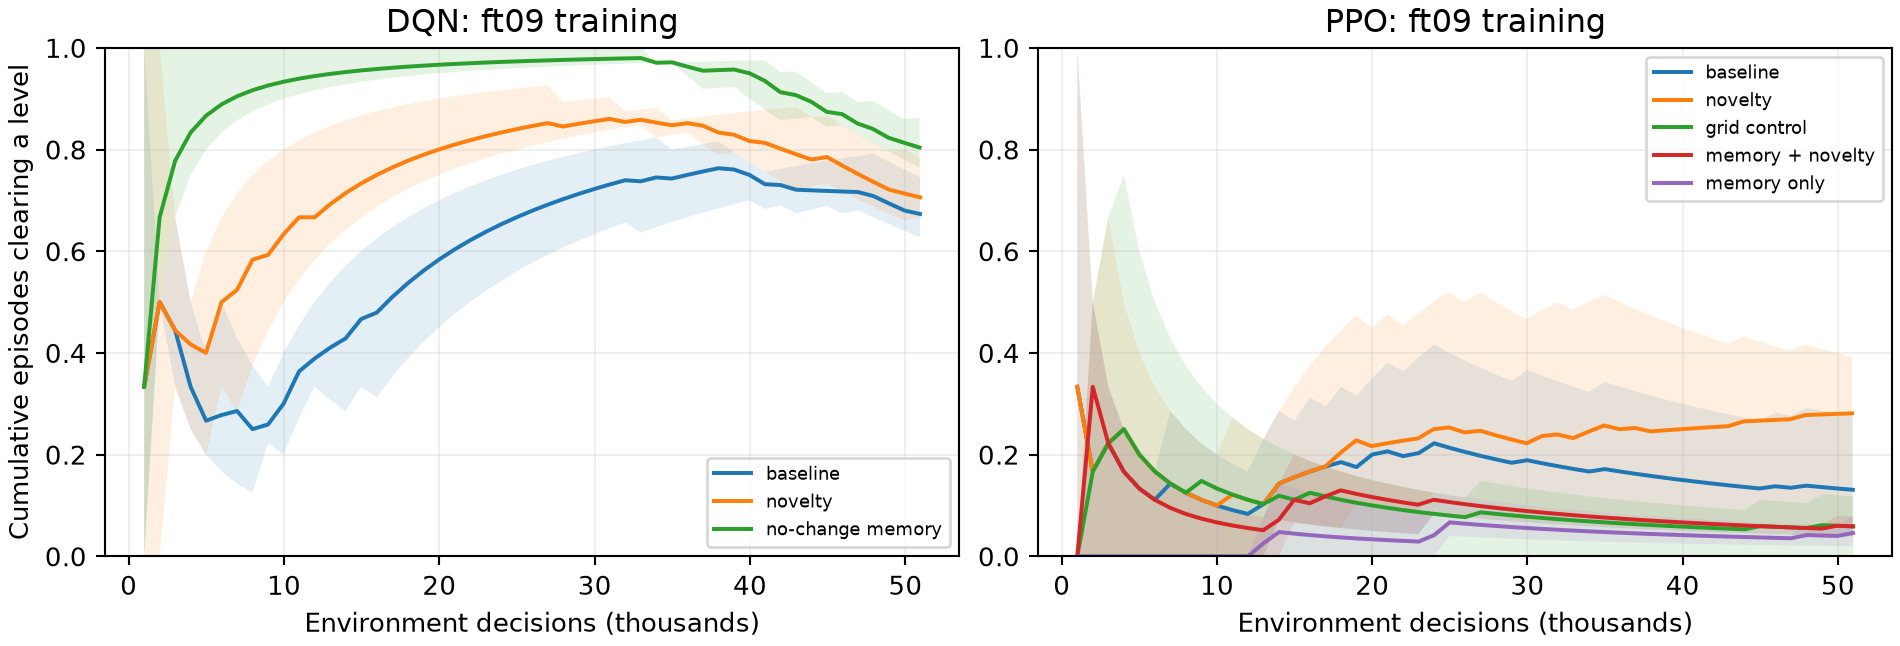
\includegraphics[width=\linewidth]{../images/learning_curves.png}
\caption{Cumulative training episodes clearing a level on ft09 against decisions. Lines are means over three training seeds; shaded regions span their minimum and maximum. These are exploratory training behaviours, not frozen evaluation or official scores. DQN training includes epsilon exploration; PPO novelty conditions also receive intrinsic reward.}
\label{fig:learning}
\end{figure}

\subsection{Comparison, variability and cost}
DQN's baseline with evaluation exploration exceeds the sampled PPO baseline and the pooled novelty-PPO result on ft09 (Table~\ref{tab:results}). This supports a narrow development comparison, not broad superiority: evaluation mechanisms differ and epsilon was tuned on development data. No DQN condition completes levels on the other three development games. PPO has zero completions on dc22 and m0r0; memory-only has one g50t completion in 60 rollouts, with all other g50t conditions at zero. Single successes do not demonstrate reliable adaptation.

All audited PPO greedy evaluations complete zero levels. Historical ft09 improved-DQN greedy files contain only one episode per seed, whereas stochastic files contain 20; these cannot support an equally precise greedy-versus-stochastic rate comparison. All audited development episodes consume their 1,000-action budget because no full-game win occurs; success counts must not hide the cost of failures. Figure~\ref{fig:learning} separates training-time progress from the weaker frozen-policy results.

Across 12 training runs per stage, completed DQN baseline, novelty and memory logs record respectively 7.34, 7.17 and 7.04 hours and approximately 609,000 decisions each. Completed PPO baseline and novelty cost 1.26 and 1.38 hours; grid-control, memory-plus-novelty and memory-only cost 1.53, 1.80 and 1.80 hours. These exclude orchestration overhead, failed attempts, smoke tests and evaluation. The evaluation CSV wall-time field is cumulative: file cost is its last value, not a sum across rows. Original logs and separate aggregate tables accompany the report. CPU DQN versus GPU PPO is an explicit hardware confound.

\section{Behavioural diagnosis and final transfer}
A sampled novelty-PPO trajectory clears ft09 level one and then makes 690 ineffective decisions. Read-only development-game inspection shows the original lattice reaches all eight first-level tiles but none of 13 second-level tiles. A 16-by-16 lattice reaches all 13. This is a structural impossibility for the original discrete action set, independent of policy quality. Coverage is necessary but not sufficient: the finer-grid control reduces first-level completion relative to novelty with grid 8. Increased exploration difficulty is plausible, but not isolated causally by this experiment.

\begin{figure}[t]
\centering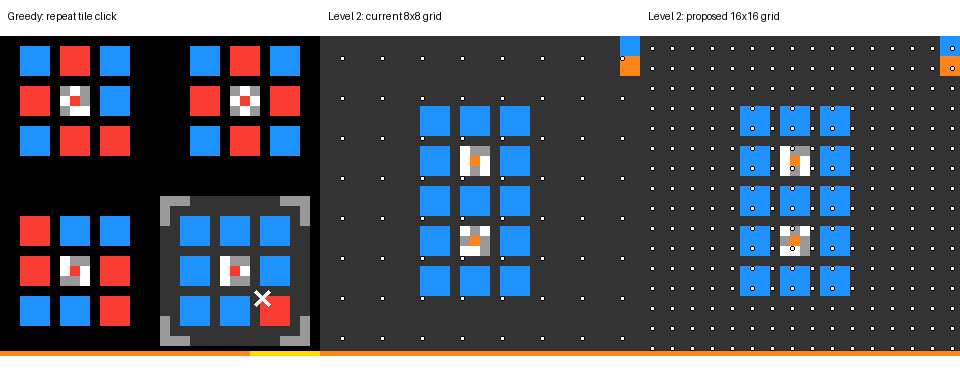
\includegraphics[width=\linewidth]{../images/diagnostic.png}
\caption{Recorded development diagnosis: a repeated tile click changes pixels without solving the puzzle (left). The second-level puzzle has no reachable tile under the 8-by-8 lattice (centre), whereas the 16-by-16 lattice reaches its tiles (right). This audit uses development source/state for interpretation, never as a policy input.}
\label{fig:diagnostic}
\end{figure}

The greedy agent's repeated colour toggling also shows why a no-change mask cannot detect every unproductive cycle: visually changing states may remain task-irrelevant. A transformer might represent longer dependencies, but architecture alone cannot repair unreachable actions or guarantee discovery from sparse success. A justified next experiment would compare reachable action abstractions and longer action-conditioned memory under matched exploration budgets.

The final transfer evaluation takes all three ft09-trained seeds of each
algorithm's baseline, novelty and final memory stage (DQN no-change memory;
PPO memory + novelty) and runs them unchanged on
cd82, tr87 and vc33. Each checkpoint plays five rollouts per game, with sampling
seeds 100--104 and the same 1,000-action budget: 270 episodes across six stages.
Five rollouts rather than 20 keep the evaluation cost manageable while retaining
all three training seeds. No held-out outcome influenced model selection or
parameters. This tests transfer from a single training game, not online
adaptation or multi-game training.

All PPO stages and both improved DQN stages complete zero levels on all three
held-out games. DQN baseline seed 1 completes one tr87 level in one of five
rollouts (one of 15 pooled baseline rollouts on tr87); its other seeds complete
none. No agent wins a game, and every episode uses its full action budget. The
single completion does not establish generalisation. Development success on one
game therefore gives little assurance of transfer to a new puzzle under this
protocol. Per-seed results and the frozen protocol are in the evidence folder.


\section{Submission, limitations and conclusion}
We package independent notebooks for three DQN stages and five PPO conditions. Every notebook embeds inference code and NumPy model weights, uses the official Agent interface and competition-provided wheels, and requires CUDA. Exported logits are checked against original PyTorch networks. The development Windows/Python 3.14 CUDA wheel is not a Kaggle dependency: inference uses the competition's Linux/Python environment and installed PyTorch. The ordinary notebook run validates inference and creates the official starter's placeholder parquet; it is not an official score. Only a competition rerun through the gateway can obtain that score.

The nominated entry is DQN baseline seed 1 with epsilon 0.3, selected from development performance before final transfer results. PPO novelty seed 2 is the principal PPO alternative. Both use an 8-by-8 grid, whose diagnosed reachability limitation remains. Models are applied unchanged to all games, with no identity-based checkpoint routing. The nominee is a selected checkpoint, not the average three-seed performance; its 20/20 development result is subject to selection bias. No model parameters adapt during competition evaluation; visual, no-change and action memory reset between games, and no information is shared across games.

The lecturer has permitted submission of the complete package through Moodle and will determine whether proxy Kaggle scoring is allowed. We therefore provide no invented submission ID or score. If proxy submission is disallowed, the lecturer's stated policy rescales the other marks. Actual competition execution and Paper Track publication must be evidenced separately from local testing.

Private development-game source/state was inspected to diagnose coverage and trajectories. Training and inference use only public observations, legal actions and past chosen actions; no held-out source, solution or scripted game-specific sequence is used. This source-informed development is disclosed rather than presented as an uninformed benchmark run. One PPO attempt failed with host-memory allocation error and was restarted; archived partial outputs are excluded. Missing historical configurations, unequal hardware, development selection, limited transfer sampling and absent official scores constrain the conclusions.

Our contribution is a reproducible two-algorithm investigation with tested, sometimes unsuccessful interventions. Exploration can produce useful first-level behaviour, but completion varies sharply by seed and does not extend to full games. Representation checks and trajectory inspection explain failures that aggregate rewards conceal. The results support more careful action design and controlled exploration studies, rather than a claim that either final agent solves ARC-AGI-3.

\section*{Contributions and AI assistance}
Nathan Le Roux: DQN implementation and experiments. Tafara Chibanda: PPO development coordination, experimental iteration and submission integration. Samuel Snyman and Joshua Snyman: setup and documentation. Claude assisted with the initial scaffold; Codex assisted implementation, debugging, analysis, packaging and writing. The authors remain responsible for verifying the code, results and attribution. Reused resources include PyTorch, NumPy, Gymnasium, arc-agi/arcengine and the official competition starter/framework; our inference architecture reproduces our trained CNN rather than using an external pretrained model.

\begin{thebibliography}{9}
\bibitem[Mnih et al.(2015)]{mnih2015} Volodymyr Mnih et al. Human-level control through deep reinforcement learning. \emph{Nature}, 518:529--533, 2015. \url{https://doi.org/10.1038/nature14236}.
\bibitem[Schulman et al.(2017)]{schulman2017} John Schulman, Filip Wolski, Prafulla Dhariwal, Alec Radford and Oleg Klimov. Proximal Policy Optimization Algorithms. arXiv:1707.06347, 2017.
\bibitem[Schulman et al.(2016)]{schulman2016} John Schulman et al. High-Dimensional Continuous Control Using Generalized Advantage Estimation. ICLR, 2016. arXiv:1506.02438.
\bibitem[ARC Prize(2026)]{arc2026} ARC Prize. ARC-AGI-3 competition documentation and official starter. \url{https://docs.arcprize.org/arc-prize-2026}; \url{https://github.com/arcprize/ARC-AGI-3-Kaggle-Starter}. Accessed 27 October 2026.
\end{thebibliography}
\end{document}
